\documentclass[16pts]{report}
\usepackage[utf8]{inputenc}
\usepackage[T1]{fontenc}
\usepackage[francais]{babel}
\usepackage{xcolor}
\usepackage[hyphens]{url}
\usepackage[hidelinks]{hyperref}
\usepackage{amsmath}
\usepackage{graphicx}
\usepackage{geometry}
\usepackage{textcomp}
\usepackage{tabularx}
\hypersetup{hypertexnames=true}
\geometry{hmargin=2.5cm,vmargin=1.5cm}

\usepackage{listings}
\lstdefinestyle{customc}{
  belowcaptionskip=1\baselineskip,
  breaklines=true,
  frame=L,
  xleftmargin=\parindent,
  language=python,
  showstringspaces=false,
  basicstyle=\footnotesize\ttfamily,
  keywordstyle=\bfseries\color{green!40!black},
  commentstyle=\itshape\color{purple!40!black},
  identifierstyle=\color{blue},
  stringstyle=\color{orange},
}
\lstset{escapechar=@,style=customc}

\usepackage{float} %Option H pour les figures, utile.

%\maketitle
%\clearpage

\begin{document}
\bibliographystyle{unsrt}
\nocite{*}

\chapter{Architecture}
\label{cha:Architecture}

Nous avons choisi de regrouper chacun de nos modules dans différents fichiers.
Au cours de notre développement, nous sommes passés par plusieurs approches
où nous n'avions pas pris en compte des éléments déjà existants pouvant être
réutilisés. Voici donc le résultat final.
\begin{figure}[H]
    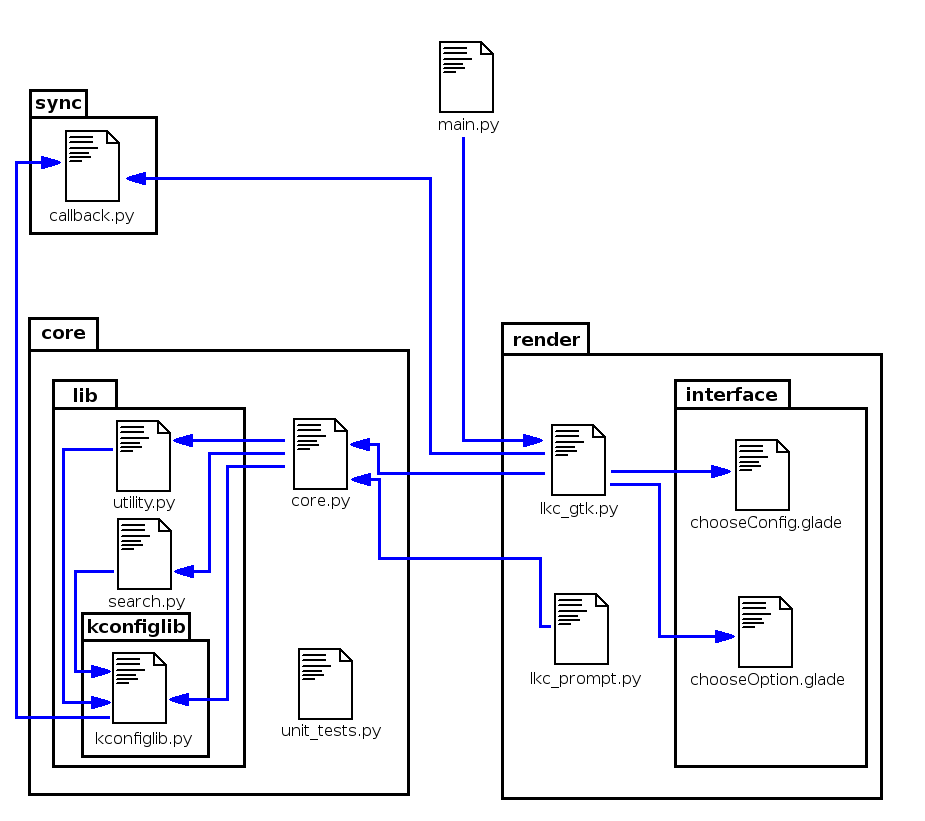
\includegraphics[scale=0.5]{illustrations/archi_add_v1.png}
    \centering
    \caption{Architecture}
    \label{fig:Arch}
\end{figure}

Les liaisons représentent les dépendances entre les différents fichiers.

\section{Décomposition modulaire}
\label{sec:Décomposition modulaire}
Notre architecture se base sur le design pattern MVVM (Model View
ViewModel) une variante du concept MVC. En effet, celui-ci contient une
partie de traitement centralisée dans le module core et son affichage dans
le module render.
La différence avec le modèle MVC, c'est qu'il n'y a pas de contrôleur.  La
plupart du temps on l'utilise pour contraindre les actions de l'utilisateur
et n'avoir que des événements souhaités. Ce qui ne nous a pas paru primordial
dans notre projet.
Notre projet contient trois modules principaux.

    \subsection{Core}
    \label{sub:Core}
    Le module core représente le \textit{modèle} de notre architecture.
    Celui-ci représente le coeur de notre application et contient
    ses principales caractéristiques.
    Il est utilisé pour l'initialisation, le parcours et le positionnement
    de valeurs d'options d'une configuration linux à générer. \\
    Ce module est lui-même décomposé en un sous-module utilisé comme
    bibliothèque interne. Celui-ci contient la bibliothèque kconfiglib, base
    de notre projet, ainsi que de deux modules utility et search nous
    permettant d'étendre les fonctionnalités de kconfiglib.
    Kconfiglib nous permet de charger en mémoire une configuration Linux
    pour une architecture donnée, modifier et d'en générer un fichier
    utilisable dans la compilation d'un noyau.
    L'utilisation de kconfiglib se fait principalement dans une arborescence
    d'un noyau Linux décompressée. Son exécution se fait à partir d'une cible
    de compilation afin de récupérer les variables d'environnement initialisées
    dans le Makefile principal du noyau Linux. \\
    Le module utility permet entre autres de faire "croire" à la bibliothèque
    kconfiglib que son exécution se fait bien dans à partir de cette cible en
    initialisant les variables d'environnement propres à son Makefile comme
    par exemple l'architecture choisie. \\
    Afin de récupérer les différentes conditions
    (prompt, default, select, reverse, additionnal) pour des pistes
    de résolutions de conflits, une idée était de parser le retour de la
    fonction \verb|__str__()| de chacun des \textit{symboles}.
    Cependant, kconfiglib avait déjà récupéré et mis en attribut des
    \textit{symboles} ces valeurs dans un format préfixe, sauf pour les
    dépendances additionnelles.\\
    Exemple pour l'option \verb|CONNECTOR|:
    \[\verb|[&&, [DM_MIRROR, NET, MD, DM_LOG_USERSPACE]|\\\]

    Sous cette forme, il est facile de créer un arbre qu'on puisse parcourir en
    profondeur pour ainsi avoir la notation infixe représentative.
    Chacun des noeuds aurait comme valeur soit un arbre, soit un opérateur
    logique (|| \&\& !) et au niveau des feuilles le nom d'un symbole.\\

    \begin{figure}[H]
        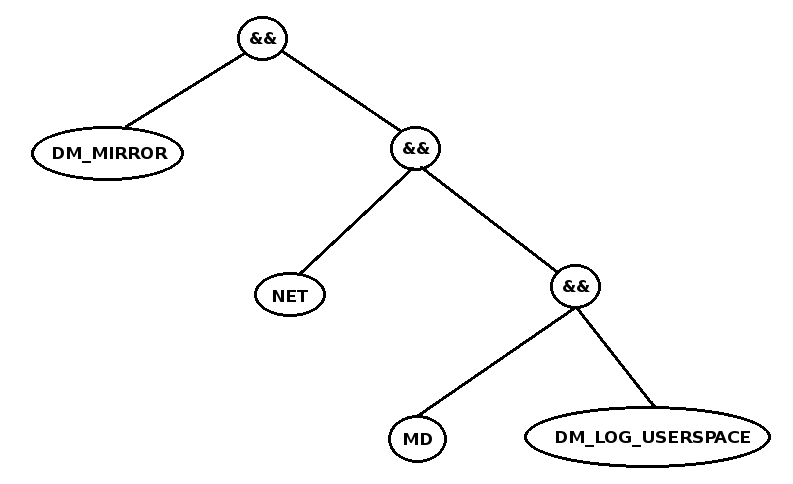
\includegraphics[scale=0.5]{illustrations/condition_tree.png}
        \centering
        \caption{Exemple d'une représentation en arbre d'une condition}
        \label{fig:condTree}
    \end{figure}

    Le module search, permet de chercher une liste d'options ayant au choix,
    dans leur nom, leur description, leur aide un mot-clé mis en entrée.

    \subsection{Render}
    \label{sub:Render}
    Le module render représente la \textit{vue} de notre architecture.
    Celui-ci représente l'interface visuelle du module core.
    Dans la version délivrée, il contient une implémentation GTK sous la forme
    de classes utilisant des fichiers XML générés avec l'outil Glade
    correspondant à nos maquettes.

    \subsection{Sync}
    \label{sub:Sync}
    L'architecture choisie rend l'application maintenable, modulaire et
    indépendante du choix de l'implémentation de l'IHM. En effet, la partie
    graphique ne fait qu'afficher l'état courant du \textit{modèle} et
    le module sync permet aux bibliothèques graphiques de mettre à jour un
    objet, tel qu'une barre de chargement. Ce mécanisme nous permet d'afficher
    l'avancement de l'initialisation du logiciel pour l'utilisateur final.

    De plus, le logiciel étant ouvert, on laisse à qui le souhaite le choix de
    modifier ou de changer le comportement proposé mais aussi d'outil
    graphique. En effet, il est possible de migrer vers une autre solution
    telle que QT, pour un choix de portabilité avancé,  ou encore ncurses, ce
    qui répondrait à un de nos besoins non fonctionnel qui était de pouvoir
    lancer l'application en mode console sur un environnement avec ou sans
    serveur X.


\end{document}
